\documentclass[journal=jacsat,manuscript=communication]{achemso}
% \documentclass{achemso}
\usepackage{mhchem}
\usepackage{siunitx}
\usepackage{float}

\title{Coding a Variational Method \& Hartree-Fock solver using Open-Source tools.}
\author{Adam Keim}
\email{a_keim@coloradocollege.edu}

\newcommand*\dif{\mathop{}\!\mathrm{d}}
\newcommand{\matr}[1]{\mathbf{#1}}

\begin{document}
\begin{abstract}
WRITE THIS LAST BUT WRITE THIS SOON 
\end{abstract}
\section{Introduction}
Most undergraduate chemistry curriculums gloss over underlying quantum mechanical principles, in large part due to the amount of mathematics required, as well as how abstract many of the ideas involved are. Despite not receiving instruction in quantum mechanics (QM) past toy systems, such as the classic (not classical!) particle in a box, many of these same students are exposed to software packages like Gaussian or WebMO, which harness the aforementioned QM principles to perform physical chemistry calculations.  By leveraging a number of computational approaches, this project aims to show the value of computational quantum methods in the classroom as a way to make computational solver packages less of a "black box."

The project presented in this work uses open-source computational chemistry methods to guide students through solving a number of quantum-mechanical systems, using both variational and Hartree-Fock methods.  All of the code is implemented in Python, and is based on the work of [REF: Meyer, Schrier].  In each case, the calculated values are compared to exact values from the literature, and in the case of the more advanced methods, further directions that students may want to take these projects are emphasized.


\section{Background}
There are a number of assumptions that we will make in all of the following cases to drastically simplify solving our system.  The first, and most important of these is that we will neglect relativistic effects, treating our momentum operator as non-relativistic.  We also employ the Born-Oppenheimer approximation, which treats atomic nuclei as static and neglects any changes in their positions.  There are a number of other assumptions which are made, which relate to how we describe wavefunctions as linear combinations of orthogonal basis functions, and that each stationary state (energy eigenfunction) of the system corresponds to one orbital.  We also note that when we are discussing the Hartree-Fock method, our discussion only applies to closed-shell systems (restricted Hartree-Fock), where all orbitals are doubly occupied. 

There are two methods that we will use to estimate energy levels for the systems we are considering.  The first of these is the variational method, a foundational tool in quantum mechanics (a detailed explanation, and justification for, this method can be found in any quantum mechanics textbook, though I am quite fond of Griffiths [REF]).  We will apply this method to a 2-nucleus \ce{H2+} molecular ion, and calculate energy levels and a bond dissociation curve.  The goals of this experiment are to lay out some of the foundational software tools that we will be using for some of the other systems, as well as showing how close of an estimate one can arrive at using quite simple methods.

The second method is the Hartree-Fock method [REF], which allows us to consider multiple electrons (as long as orbitals are filled, remember this is \textbf{Restricted} Hartree-Fock).  

\section{Experimental}
\subsection{Variational solution of a 2 Nucleus system}
The first choice that needs to be made to analyze the two nucleus \ce{H2+} molecular ion is that of a suitable coordinate system.  In this work, confocal ellipsoidal coordinates are used, where the two foci of the ellipse are given by the two nuclei.  This gives a Hamiltonian operator (an operator from quantum mechanics that describes the total energy of a system) of
\begin{equation}
	\hat{H} = \frac{-2}{R^2\left(\xi^2-\eta^2\right)}\left[\left(\xi^2-1\right)\frac{\partial^2 }{\partial\xi^2}\right]-\frac{2}{R(\xi+\eta)}-\frac{2}{R(\xi-\eta)}+\frac{1}{R}.
\end{equation}
To apply the variational method [REF GRIFFITHS], a trial wavefunction needs to be selected, and in this case a reasonable choice is
\begin{equation}
	\phi_t = c\left(\frac{Z^{3/2}}{\sqrt{\pi}}e^{-Zr_a} + \frac{Z^{3/2}}{\sqrt{\pi}}e^{-Zr_b}\right).
\end{equation}
Where c is a constant
With the Hamiltonian and a trial wavefunction, we can apply the variational method.  Since our trial wavefunction is not necessarily normalized, this looks like
\begin{equation}
E_{ground} \leq \frac{\left<\phi | \hat{H} | \phi \right>}{\left<\phi|\phi\right>}.
\end{equation} 
The angular bracket notation is known as bra-ket notation and is a standard notation commonly used in quantum mechanics, where
\begin{align}
	\left<x|y\right> &= \int x^* y d\tau \\
	\left<x|\hat{O}|y\right> &= \int x^* \hat{O}yd\tau.
\end{align}
\subsection{Self-consistent calculations for He atom}
For an \ce{He} atom, things get a little more complicated.  There are no known analytic solutions for systems of more than one electron, so even the best solutions still have errors in their approximations.  However, since there is only one nucleus, there is no need to introduce the concept of basis sets, and we can use Slater-type \textit{1s} functions with the form 
\begin{equation}
	\phi_n(r,\theta,\phi) = 2\zeta_n^{3/2}e^{-\zeta_nr/a_0}Y_0^0(\theta,\phi)
\end{equation}
where $\zeta$ is a parameter that describes the spatial extent of the function.  Optimal values for $\zeta$ are selected according to [REF].  The method used to evaluate the wavefunction is known as the Hartree-Fock method, and consists of the following major steps:
\begin{enumerate}
	\item Choose the number of occupied orbitals $N_\mathrm{occ}$, number ($N_\mathrm{basis}$), and type of bases.
	\item Calculate overlap, orthogonality transform, one-electron, and two-electron matrices.  For both of our choices of basis set, we can calculate these analytically ahead of time rather than numerically.
	\item Make initial guesses for eigenvector coefficients and use these to calculate a charge density matrix, given by
\begin{equation}
	P_{tu} = 2 \sum_{i=1}^{N_{\mathrm{occ}}}c^*_{it}c_{iu}.
\end{equation}
	This matrix describes where the electrons are located in terms of our bases.
	\item Build our Fock matrix $F_{rs}$ following

\begin{equation}
	F_{rs} = h_{rs} + \sum_{t=1}^{N_\mathrm{basis}}\sum_{u=1}^{N_\mathrm{basis}}P_{tu}\left\{(rs|tu) -\frac{1}{2}(ru|ts)\right\}.
\end{equation}
	\item Calculate $\matr{F}' = \matr{X}^\dag\matr{F}\matr{X}$.
	\item Solve the eigensystem $\matr{F}'\vec{c'}_i=\epsilon_i\vec{c'}_i$.
	\item Transform back to our original basis $\vec{c}_i$
	\item Build a new charge density matrix, $\matr{P}$ from eigenvectors obtained in previous step.
	\item If the difference in energy 
\begin{equation}
	E = \sum_{i=1}^{N_\mathrm{occ}}\epsilon_i + \frac{1}{2} \sum_{r=1}^{N_\mathrm{basis}} \sum_{s=1}^{N_\mathrm{basis}}P_{rs}h_{rs}+V_{nn}
	\label{eq:hf_energy}
\end{equation}
is smaller than some threshold, terminate.  Otherwise, go back to step 4.
\end{enumerate}

Practically, we don't define a threshold for Step 9, since the systems we are interested are small enough that they converge after $<10$ iterations. 


\subsection{Self-consistent calculations for \ce{H2}}
Once there are two nuclei in the system, Slater-type orbital functions get messy, so we approximate the orbital wavefunctions as a linear combination of Gaussian-type orbitals, to both speed up and simplify the following calculations.  A $1s$ Gaussian basis function is given by
\begin{equation}
	g_{1s}(\vec{r}_\alpha)=\left(\frac{2\alpha}{\pi}\right)^{3/4}e^{-\alpha|\vec{r}_\alpha|^2},
\end{equation}
which has the familiar form of a Gaussian distribution, and is quite simple to integrate analytically.  The only other thing that changes relative to the previous experiment, other than basis sets, is that there is now a contribution to the energy from the Coulombic repulsion between the two nuclei, which must be taken into account. (The $V_{nn}$ term in Equation \ref{eq:hf_energy})  Otherwise, the self-consistent field calculations remain similar, and we are able to calculate a ground state energy and a bond dissociation curve.
\section{Results and Discussion}

{\setlength{\extrarowheight}{2pt}
\begin{table}[H]
  \begin{tabular}{l|ccc}
    Property & Variational Method & Exact & \% Error \\
    \hline
    $R_e$ (\si{\angstrom}) & 1.060 & 1.057 & .28\%\\
    $E$ (\si{\hartree}) & -.5865 & -.6026 & 2.67\%
  \end{tabular}
  \caption{Results for the variational method.  Exact values from [REF Meyer].  $R_e$ is the equilibrium bond length, and $E$ is the ground state energy. }
  \label{tab:var}
\end{table}

Table \ref{tab:var} compares the values obtained from the variational method to exact values from the literature, and we see that the values are in quite good alignment, to within $<3\%$.  Unfortunately, the variational method is limited to systems of one electron, though we can still obtain an energy contour plot showing the variational energy across $R,Z$ space.  By taking the minimum energy for each $R$, we obtain a bond dissociation curve (Figure \ref{fig:var_bd}), which has the characteristic shape that we expect to see for a curve of this type.  [REF INTRO CHEM TEXTBOOK]

\begin{figure}[H]
  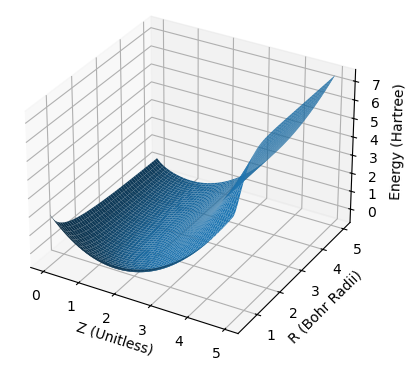
\includegraphics[width=.5\textwidth]{figures/variational_energy_contour.png}
  \caption{Energy contour plot for the \ce{H2+} molecular ion, calculated with the variational method.}
\end{figure}



\begin{figure}[H]
  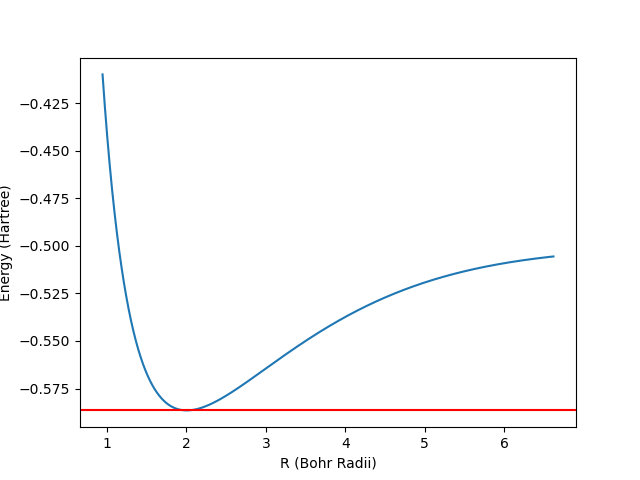
\includegraphics[width=0.5\textwidth]{figures/variational_dissociation.png}
  \caption{The bond dissociation curve for the \ce{H2+} molecular ion, calculated with the variational method.}
  \label{fig:var_bd}
\end{figure}

{\setlength{\extrarowheight}{2pt}
\begin{table}[H]
  \begin{tabular}{l|ccc}
    Property & Hartree-Fock & Exact & \% Error \\
    \hline
    $R_e$ (\si{\angstrom}) & .78 & .74 & 5.4\%\\
    $E$ (\si{\hartree}) & -.5865 & -.6026 & 2.67\%
  \end{tabular}
  \caption{Results for the variational method.  Exact values from [REF Schrier].  $R_e$ is the equilibrium bond length, and $E$ is the ground state energy. }
  \label{tab:hf}
\end{table}

\begin{figure}[H]
  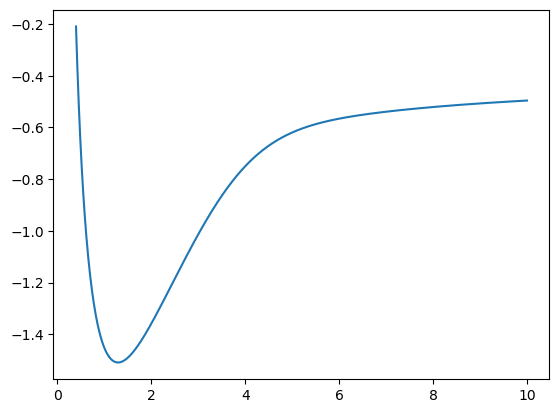
\includegraphics[width=0.5\textwidth]{figures/Bond_Dissociation_Hydrogen.png}
  \caption{The bond dissociation curve for the \ce{H2} molecule, calculated with Hartree-Fock methods.}
\end{figure}

\section{Conclusion}
Coding is a proven method to increase feelings of gratification experienced by students while learning[REF].  Abstract concepts such as quantum mechanics lend themselves particularly well to computational methods, given the heavy mathematics and abstract concepts involved.  By providing students with a sequence of experiments which they can carry out in the classroom, this work aims to "de-mystify" some of the quantum-motivated computations happening inside of computational chemistry packages such as Gaussian and WebMO. The tools used for the computations are exclusively open-source, with hopes that students who do not have access to, or do not wish to use, proprietary software packages like Mathematica can study and replicate these experiments as an method to further their chemistry education. Overall, this project aims to point students at a number of projects they can carry out, as well as providing Python code to assist in debugging and verifying results. 

\section{Further Directions}
There are a number of quite interested further directions for this research.  Interested students could generalize the Hartree-Fock code to either treat systems with more numerous nuclei or electrons, or remove the restriction on our Hartree-Fock implementation that forces completely full orbitals.  It would also be interesting to add more complex gaussian basis sets to better describe the spatial extent of the wavefunction of electrons, recalling that this will approach an asymptotic Hartree-Fock limit.  Modern approaches to similar problems often either exclusively use, or combine with Hartree-Fock, methods known as density functional theory (DFT), which is an exact method that does not have an instrinsic limit, and is limited by our approximations about physical systems.  
\end{document}